\documentclass{article}
\usepackage{cmap}
\usepackage[utf8]{inputenc}
\usepackage[english,ukrainian]{babel}
\usepackage{graphicx}
\usepackage{geometry}
\usepackage{listings}
\usepackage{float}
\usepackage{amsmath}
\usepackage{subfig}
\usepackage{xcolor}
\geometry{
	a4paper,
	left=20mm,
	right=20mm,
	top=15mm,
	bottom=15mm,
}
\lstset{
	tabsize=4,
	keepspaces,
	showstringspaces=false,
	escapeinside={(*@}{@*)},
	breaklines,
}
\graphicspath{ {./pictures} }
\setlength{\parindent}{4em}

\newcommand\subject{Архітектура комп'ютера}
\newcommand\lecturer{доцент кафедри ПЗ\\Крук О.Г.}
\newcommand\teacher{доцент кафедри ПЗ\\Крук О.Г.}
\newcommand\mygroup{ПЗ-22}
\newcommand\lab{11}
\newcommand\theme{Використання цифрових портів мікроконтролера STM32F401RB}
\newcommand\purpose{Опанувати роботу з цифровими портами мікроконтролера STM32F401RB; розвинути навики складання програми мовою С для виведення і введення сигналів через цифрові порти; відтранслювати програму, складену відповідно до свого варіанту в середовищі програмування Keil uVision MDK-ARM; виконати моделювання схеми з мікроконтролером в системі Proteus}

\begin{document}
	\begin{normalsize}
		\begin{titlepage}
			\thispagestyle{empty}
			\begin{center}
				\textbf{МІНІСТЕРСТВО ОСВІТИ І НАУКИ УКРАЇНИ\\
					НАЦІОНАЛЬНИЙ УНІВЕРСИТЕТ "ЛЬВІВСЬКА ПОЛІТЕХНІКА"}
			\end{center}
			\begin{flushright}
				\textbf{ІКНІ}\\
				Кафедра \textbf{ПЗ}
			\end{flushright}
			\vspace{200pt}
			\begin{center}
				\textbf{ЗВІТ}\\
				\vspace{10pt}
				до лабораторної роботи № \lab\\
				\textbf{на тему}: “\textit{\theme}”\\
				\textbf{з дисципліни}: “\subject”
			\end{center}
			\vspace{112pt}
			\begin{flushright}
				
				\textbf{Лектор}:\\
				\lecturer\\
				\vspace{28pt}
				\textbf{Виконав}:\\
				
				студент групи \mygroup\\
				Коваленко Д.М.\\
				\vspace{28pt}
				\textbf{Прийняв}:\\
				
				\teacher\\
				
				\vspace{28pt}
				«\rule{1cm}{0.15mm}» \rule{1.5cm}{0.15mm} 2022 р.\\
				$\sum$ = \rule{1cm}{0.15mm}……………\\
				
			\end{flushright}
			\vspace{\fill}
			\begin{center}
				\textbf{Львів — 2022}
			\end{center}
		\end{titlepage}
		
		\begin{description}
			\item[Тема.] \theme.
			\item[Мета.] \purpose.
		\end{description}
		
		\section*{Індивідуальне завдання}
		\begin{figure}[H]
			\centering
			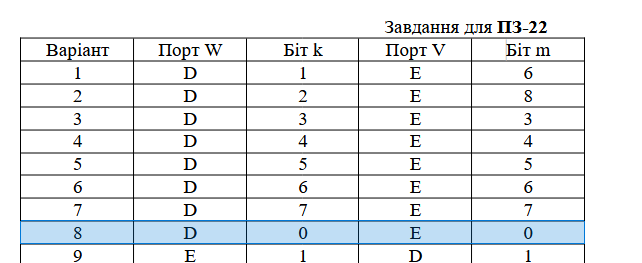
\includegraphics[scale=0.7]{2}
		\end{figure}
		
		\section*{Хід роботи}
		\subsection*{Код програми}
		\begin{lstlisting}
#include "stm32f4xx.h"
#include "stm32f4xx_gpio.h"

static __IO uint32_t uwTimingDelay;
RCC_ClocksTypeDef RCC_Clocks;

static void Delay(__IO uint32_t nTime);
static GPIO_InitTypeDef gpio_d;
static GPIO_InitTypeDef gpio_e;

int main(void) {
	RCC_AHB1PeriphClockCmd(RCC_AHB1Periph_GPIOD | RCC_AHB1Periph_GPIOE, ENABLE);
	
	GPIO_StructInit(&gpio_d);
	gpio_d.GPIO_Pin = GPIO_Pin_0;
	gpio_d.GPIO_Mode = GPIO_Mode_IN;   
	GPIO_Init(GPIOD, &gpio_d); 
	
	RCC_AHB1PeriphClockCmd(RCC_AHB1Periph_GPIOB, ENABLE); 
	GPIO_StructInit(&gpio_e);
	gpio_e.GPIO_Pin = GPIO_Pin_0;
	gpio_e.GPIO_Mode = GPIO_Mode_OUT;   
	GPIO_Init(GPIOE, &gpio_e);  
	while (1) {
		if(GPIO_ReadInputDataBit(GPIOD,GPIO_Pin_0) == 0) 
		GPIO_SetBits(GPIOE,GPIO_Pin_0);
		else
		GPIO_ResetBits(GPIOE,GPIO_Pin_0);
	}
}

void Delay(__IO uint32_t nTime) { 
	uwTimingDelay = nTime;
	
	while(uwTimingDelay != 0);
}

void TimingDelay_Decrement(void) {
	if (uwTimingDelay != 0x00) 
	uwTimingDelay--;
}

		\end{lstlisting}

\begin{figure}[H]
	\centering
	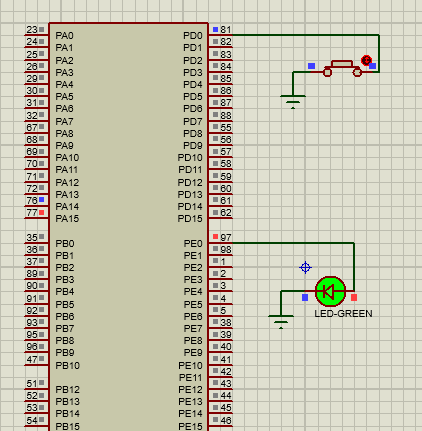
\includegraphics[scale=0.7]{1}
	\caption{Результат обчислення}
\end{figure}

			
		\section*{Висновки}
		Під час виконання лабораторної роботи я опанував роботу з цифровими портами мікроконтролера STM32F401RB; розвинув навики складання програми мовою С для виведення і введення сигналів через цифрові порти; відтранслював програму, складену відповідно до свого варіанту в середовищі програмування Keil uVision MDK-ARM; виконав моделювання схеми з мікроконтролером в системі Proteus.
		
	\end{normalsize}
\end{document}